%%%%%%%%%%%%%%%%%%%%%%%%%%%%%%%%%%%%%%%%%
% University/School Laboratory Report
% LaTeX Template
% Version 3.1 (25/3/14)
%
% This template has been downloaded from:
% http://www.LaTeXTemplates.com
%
% Original author:
% Linux and Unix Users Group at Virginia Tech Wiki 
% (https://vtluug.org/wiki/Example_LaTeX_chem_lab_report)
%
% License:
% CC BY-NC-SA 3.0 (http://creativecommons.org/licenses/by-nc-sa/3.0/)
%
%%%%%%%%%%%%%%%%%%%%%%%%%%%%%%%%%%%%%%%%%

%----------------------------------------------------------------------------------------
%	PACKAGES AND DOCUMENT CONFIGURATIONS
%----------------------------------------------------------------------------------------

\documentclass{report} %report

\usepackage[version=3]{mhchem} % Package for chemical equation typesetting
\usepackage{siunitx} % Provides the \SI{}{} and \si{} command for typesetting SI units
\usepackage{graphicx} % Required for the inclusion of images
\usepackage{hyperref}

\usepackage{amsmath} % Required for some math elements 
\usepackage{indentfirst}
\usepackage{dirtytalk}
\usepackage{titlesec}

\title{Enhancing Hearthstone deck building with a Generative Adversarial Network (GAN)} % Title
\titleformat{\chapter}{\normalfont\LARGE\bfseries}{\thechapter.}{18pt}{\LARGE\bfseries}
\titleformat*{\subsection}{\large}
\titleformat*{\subsubsection}{\normalfont}
\author{Callum \textsc{Roberts}} % Author name
\setcounter{secnumdepth}{4}


\renewcommand{\labelenumi}{\alph{enumi}.} % Make numbering in the enumerate environment by letter rather than number (e.g. section 6)
\bibliographystyle{IEEEtran}
%\usepackage{times} % Uncomment to use the Times New Roman font

%----------------------------------------------------------------------------------------
%	DOCUMENT INFORMATION
%----------------------------------------------------------------------------------------



\author{Callum \textsc{Roberts}} % Author name

\date{\today} % Date for the report

\begin{document}

\maketitle % Insert the title, author and date

% If you wish to include an abstract, uncomment the lines below
% \begin{abstract}
% Abstract text
% \end{abstract}

%----------------------------------------------------------------------------------------
%	SECTION 1
%----------------------------------------------------------------------------------------
\begin{abstract}

\end{abstract}

\section*{Acknowledgements}
Thanks Mum.

\tableofcontents

\chapter{Introduction}
\section{Overview}
Bringing Artificial Intelligence to Hearthstone: Heroes of Warcraft is not a new concept, it has been subject to many studies in the field, where it be playing the game, suggesting moves to the player or building decks. Focusing on the field of deck building, it is a concept that exists across multiple trading card games such as Magic: The Gathering, Pokemon, Yu-Gi-Oh and of course Hearthstone. Papers have studied these games more or less, but all seem to gravitate around similar deck building techniques, details of which will be expanded later on. These techniques seemingly been saturated, newer studies apply small scale changes to already defined methods (cite a paper about GAs). Exploration of different techniques has been touched on but they seem to be outliers and of limited number (cite NN paper), experimenting with other algorithms could show better, more  interesting results instead of assuming that one saturated method is the best because of its popular usage.
\section{Motivation}
Using a Artificial Intelligence algorithm that has not been utilised nor researched in the field of deck building could provide insight into the Generative Adversarial Network (GAN) applications in other fields of research, as it is mostly limited to image generation. Along with this discovering another method for deck building that could bear fruit to similar or improved results, opening the way for more techniques and deeper research into the use of recorded data for deck generation. 
\section{Aims and Objective}
The aim of this project is to create a deck building artificial intelligence using a Generative Adversarial Network (GAN) and testing the viability of it, this will be achieved by completing the following objectives:
\begin{itemize}
  \item Collecting user deck data from reliable sources
  \item Cleansing of user deck data
  \item Converting user deck data to vectors and back to human readable after training
  \item Implement GAN for single dimensional vector generation
  \item GAN hyper-parameter and layer optimization
  \item Simulating results against user decks
  \item Performing evaluations on resulting decks
\end{itemize}
\section{Key Findings}
This project has exhibited that it is possible to use Generative Adversarial Networks to generate decks for Hearthstone, a technique that seemingly no one has attempted to use, the AI demonstrates similarities to user created decks such as card types, type percentage, card duplicates, synergies and card spread. The decks tested have an average of 55\% win rate, varying from class to class, match ups against other classes greatly influenced the outcome of a match. Although the win rate is heavily influenced by the AI playing it, considering that the simulator game playing AI will not play as well as a human player. The training process is much faster than anticipated (around 10 minutes), however the testing was much longer at around 1 - 2 hours depending of the number of decks created.
\section{Structure}
The structure of the report is as follows, first a literature review which presents an overview of Hearthstone, some of the important game mechanics and existing AI that have been used. Then a discussion  of  the  requirements  of  the  project  and  the  methodology  to implement them. Following this is a discussion of the potential legal and ethical issues with the project and what has been done to overcome them. The implementation of the project, a deep dive into how the project was completed. A testing and evaluation section describing the strategy and the results of the generated decks. Finally, a conclusion which summarises the project is given.

\chapter{Literature Review}
The purpose of this literature review is to define the technologies used in the field of artificial intelligence for building a deck in Hearthstone. To introduce, and compare previous works to determine their strengths and weaknesses. A review of the literature is valuable in understanding important aspects of a research area \cite{Isaacs2020}. The structure of this literature review is as follows: the initial section will detail the background of the project, explaining the fundamentals of Hearthstone and deck building. Following that will be an introduction to the project,  motivations, and research questions. Finally, we will have the core technologies used for similar projects.
\section{Background}
	For the benefit of the reader, this section will introduce the basics of Hearthstone. It will emphasize the deck building aspect of the game including practices used by players.  
\subsection{Collectible Card Games}
	Collectible Card Games (CCG)\footnote{\url{https://en.wikipedia.org/wiki/Collectible_card_game}} are a sub-genre of card games introduced in 1993 by Magic: The Gathering \footnote{\url{https://en.wikipedia.org/wiki/Magic:_The_Gathering}}. They require players to make a custom decks to play, they mix trading cards with strategy and deck building features. CCGs are usually defined as a turn-based game, where each player acquires their own collection of cards through the purchasing of "starter decks" for beginners or "booster packs" containing a small number of random cards from a {\it{pool}} of cards usually referred to as an expansion. The aim is to build an efficient deck that can account for the inconsistency that comes from the nature of card games, to predict and play around your opponent's actions to ultimately beat them. Some CCGs can prove to be lucrative for players as cards have a value intrinsic to their rarity and demand \footnote{\url{https://www.cardmarket.com/en/Magic/}}, this makes building the perfect deck rather difficult and usually costly.
\subsection{Hearthstone}
	Hearthstone: Heroes of Warcraft is a CCG developed by Blizzard Entertainment in 2013 \cite{HS}, but with the twist of it being entirely digital, there is no physical version of the game. This choice unlocks potential for gameplay features that could not be implemented, in exchange for the tradability of cards. \\ 
\begin{figure}[h]
\centering
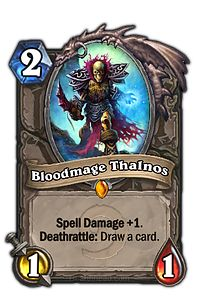
\includegraphics[width=0.25\textwidth]{thalnos}
\caption{Example of a Legendary Hearthstone card\protect\footnotemark
\label{card}
}
\end{figure}
\footnotetext{\url{https://www.pinterest.fr/pin/573716440004576557/}}

	\indent Two players face off wielding each a deck of their own making. Decks consist of exactly 30 cards. Players then take it in turns to play their cards, the objective being to reduce the other player's health to zero. On each player's turns that player draws a card and gains a “Mana Crystal” up to a maximum of 10 (crystals are refreshed every turn), these crystals are expended to cast a card from the player's hand. Before a match each player chooses to embody a class (such as Mage, Warrior, Rogue, Druid, etc…), each class has specific cards only they can add into their deck, these are adequately named “Class Cards”, these are accompanied by “Neutral Cards” that any class can use. Classes also have access to an ability unique to them called a "hero power". \\
	
\begin{figure}[h]
\centering
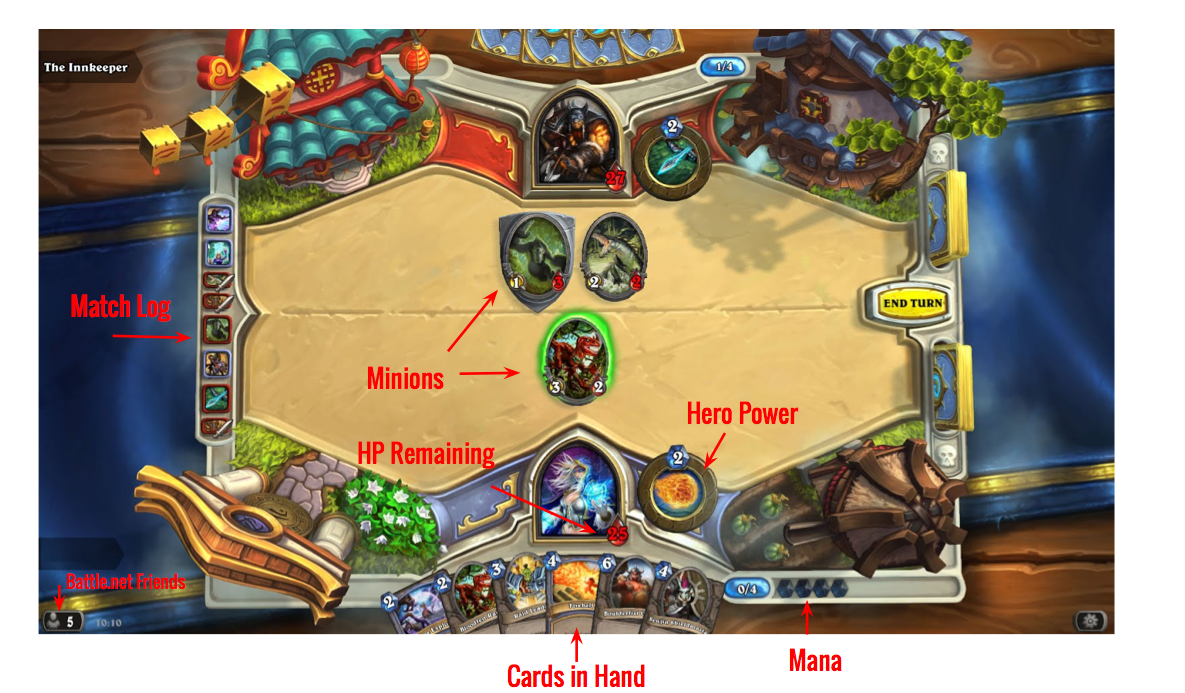
\includegraphics[width=1\textwidth]{hearthstonegameboard}
\caption{Example of a Hearthstone board\protect\footnotemark}
 \label{board}
\end{figure}
\footnotetext{\url{https://bothgunsblazingblog.wordpress.com/2014/06/22/hearthstone-analysis-and-deconstruction/}}
	
	Each card in the game has a “mana” cost which shows how many mana crystals are needed to cast that card. They also have a card type, rarity, and an effect. In a deck, players can put duplicates of the same card (up to 2) except for "Legendary Cards" (figure \ref{card}) that are limited to a single copy due to their powerful effects.  Players have a “Collection”, where the cards they own are stored, to get new cards players can buy card packs with gold, the in-game currency of Hearthstone. Gold is earned slowly through quests, winning, and events, however this process can be sped up through the purchase of gold with real-life currency. Players can also choose to "Disenchant" their duplicate cards to gain another in-game currency called "Dust" which can be used to create a card of the players choosing\footnote{\url{https://hearthstone.gamepedia.com/Crafting}}.


\subsection{Deck Building}
	In the world of CCGs, there is a long-standing debate on how to measure the skill of a player. Although card games involve luck and circumstance, it is believed that there is a degree of strategy in the building and execution of decks whether it is just a slight increase in win probability or a fundamental to winning \cite{SvsL}. However, the debate stems from which is the most important, the building aspect or the execution aspect of CCGs.
	\cite{BvsP}
	\subsubsection{Metagame}
	Hearthstone is a game with lots of complex systems that are influenced by many factors, mainly due to a large number of cards and different playable heroes. In a game where there are lots of variables, players try to rank cards, heroes, and combinations to increase their chances to win. This phenomenon creates decks from a "pool" of top-rated cards, leaving out the mediocre, forcing players to use these top-rated decks in order to have a better chance of winning or be put at a disadvantage. The result is what is called the "Metagame" or {\it{meta}} for short\footnote{\url{https://www.hearthstonetopdecks.com/hearthstones-best-standard-ladder-decks/}}. Blizzard release updates to the game frequently through "expansions"\footnote{\url{https://hearthstone.gamepedia.com/Expansion}} which add a variety of new cards to keep the game fresh. Shifts in the meta occur when these expansions are added and players experiment to find better combinations over time. However better cards may not be added, and changes in the meta may not occur, this dissuades players from continuing or returning to play knowing that they have already experienced all that they can. To avoid that Hearthstone has implemented two-game modes\footnote{\url{https://hearthstone.gamepedia.com/Game_format}}, one in which only cards added over the past two years are available, and another mode that allows all cards. Whilst this method has helped, it still does not put a stop to the possibility of a stale meta. Researchers have done studies on how to evolve the meta through AI means, by {\it{balancing}} powerful cards ({Fernando et al.}) \cite{EvolveMeta}. Balancing a card means to adjust the power of said card to make it more or less viable in the current game environment. Fernando et al. discussed the idea that around 50\% of Hearthstone's meta is derived from match-ups which is the win probability two decks have against each other, a favorable match-up being the one with the highest win probability or known in the community as {\it{win rate}}.  
\subsubsection{Mana Curve}
	Theorycrafting is a term used widely in many video games, it designates a mathematical analysis of a game's core mechanics to attempt to discover new strategies or combinations that could rival the current ones. Hearthstone is one such game, a large portion of the player base enjoys theorycrafting new decks that may {\it{break}} the meta, as in cause a fundamental shift of the current metagame. These players rely on fundamentals or schematics that are used as a guideline in building a new deck. The {\it{mana curve}} \footnote{\url{http://hearthstone.gamepedia.com/Mana_curve}} is one such fundamental, it exists in all decks built in the game. Every card in Hearthstone has a cost, this cost determines the power of the card, a low-cost card will be weaker than a higher cost card since it would cost fewer resources to cast. This {\it{mana curve}} is a histogram of each card plotted by cost, it allows players to visualize how expensive in resources their deck is and to determine the deck's archetype. 
\begin{figure}[h]
\centering
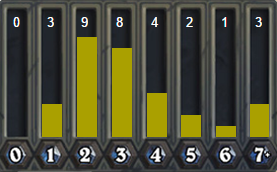
\includegraphics[width=0.5\textwidth]{mana_curve}
\caption{Example of a Mana Curve\protect\footnotemark}
\label{board}
\end{figure}
\footnotetext{\url{https://hearthstone.judgehype.com/deck-mage-tempo-ladder-legendaire-tgt-gvg/}}
\subsubsection{Archetype}
\label{archetypes}
	The word archetype is derived from the Greek word {\it{archétypon}} which means "beginning, origin", applied in the psychology field to categorize complex human behaviour called "Jungian Archetypes" \cite{Robertson2016}. This term was transposed into the deck building field of CCGs, a deck's archetype is meant to categorize and describe the behaviour of the deck from a high-level perspective, forgoing the need to play the deck to learn its strategy. In Hearthstone, most decks can be categorized by three main archetypes \cite{Judlick}:
\begin{itemize}

\item \textit{Aggro} decks are the aggressive decks meant to defeat an opponent as quickly as possible, as a consequence the mana curve of such decks is focused towards the cheaper side of the histogram. Their power comes in the early turns, but they quickly become weaker to the other archetypes as the turns go on.
\item \textit{Control} decks are meant to control the state of the board through the use of expensive cards, they tend to generate a lot of cards and have a wide range of card choices. The mana curve of such an archetype is towards the expensive end of the histogram. They tend to have a few cards to play early in the game but have a multitude of win conditions in later turns.

\item \textit{Mid-range} decks are situated in the middle of the two other archetypes, focusing mainly on the mid-game, their win conditions are stronger than the aggro decks but weaker than the control decks. Their mana curve peaks in the middle of the histogram.
\end{itemize}

Hearthstone also has other archetypes that cover a shorter scale, they are usually introduced in the newer expansions and rotate out of the normal game after a couple of years \cite{Standard}. For example, a highlander archetype is a deck with 30 unique cards. Archetypes are formed around specific cards with win conditions\footnote{\url{https://playhearthstone.com/en-us/news/21363038}}, meaning that they have the power to win the game. So in the example given in a highlander deck, there would be a card that has an effect that triggers from having only unique copies in the deck.
 
\subsubsection{Resource Cost}
	In CCGs, cards have a certain cost to use, in Hearthstone that cost is mana which regenerates every turn. The cost of a card is determined by the power of said card, if it has a powerful effect, has decent attack and defence values, or even both. This cost will determine how late into the game a card can be played. However, a card that costs a lot can be considered weak and a low-cost card can be considered strong. The power of a card is determined through the resource cost, an invisible value that is hard to calculate and a subject of study \cite{Zuin2019}. Although the Zuin et al. study was used to predict the cost of a card in Magic: The Gathering, the resource calculation is still present in Hearthstone. It poses a good solution to the balancing of the metagame and would be adaptable to Hearthstone. A card is considered efficient if the theoretical resource cost is higher than the current mana cost, and would be inefficient if the resource cost were to be lower than the mana cost. The resource cost of a card is something that may need to be considered when developing an AI for building decks. Stiegler et al. \cite{Stiegler2017} applied a similar theory to design a deck-building AI based on a utility system that classified cards based on resource cost-effectiveness, mana curve, and synergies.
\section{Project Introduction}
	 The rising popularity of Hearthstone has attracted a lot of new players reaching over 100 million accounts in 2018 \cite{100mil}, however, due to the nature of collecting cards in the game some will not have the required cards to build the most popular decks. The game is free, anyone can download it, however, a lot of the content is locked behind a paywall\footnote{\url{https://en.wikipedia.org/wiki/Paywall}}. Whilst it is possible to earn cards by earning "gold", it becomes a time-consuming ordeal that requires a lot of spare time to invest. With new expansions being added regularly, the game seems to become a never-ending grind, unless you decide to pay real money to acquire currency. This is where the term "pay-to-win" is used to describe Hearthstone \cite{Howard2019}, meaning that to get the most enjoyment and the highest chance to win, the player must spend money or be disadvantaged. The goal of this honours project is to create an AI that builds decks from a  collection of cards, incomplete or otherwise in order to improve the game experience for players that are unable or not willing to pay. For players that do own a large collection of cards, it can also provide fresh new decks to play that differ from the more popular ones.
\subsection{Related Works}
	Video games are the ideal tool for the training of Artificial Intelligence. The virtual space that a game provides is a realistic environment with a limited amount of information available \cite{Sweetser2002} allowing control and knowledge over the behaviour of the AI. Hearthstone is a game that provides a platform for a wide variety of AI that differs from AI-benchmark games such as Chess or Go. Hoover et al. \cite{Hoover2020} classifies Hearthstone AI into specialized categories: 
\begin{itemize}
\item Game Playing AI, rather self-explanatory, this form of AI is designed to play the game. Generally, tree search algorithms are used, Monte Carlo Tree Search (MTCS) in particular. However, this method is rather ineffective in Hearthstone due to the amount of hidden information and limited visibility of the AI. Developers of Hearthstone simulators, such as {\it{MetaStone}}\footnote{\url{http://www.demilich.net/}} tend to use a greedy approach to compensate \cite{Yannakakis2018}. Some researchers attempt to use variations of MCTS and heuristics to work around the limited information \cite{Janusz2017}\cite{Santos2017}\cite{Swiechowski2018}.
\item Developer Assisting AI, this AI help with certain issues that developers could have. Since Hearthstone has hundreds of cards, it is challenging to design cards with new flavour that are not identical to previously printed cards. Could there be a way to generate inspiration? Woolf "minimaxir" Max\footnote{\url{https://minimaxir.com/apps/gpt2-mtg/}} created an API that generates Magic: The Gathering cards\footnote{For example cards: \url{https://github.com/minimaxir/mtg-gpt-2-cloud-run/tree/master/generated_card_dumps}} using a transformer language model\footnote{\url{https://openai.com/blog/tags/gpt-2/}} for such a purpose. Another possible use is for balancing the game, since maintaining game balance when creating additional cards may create unfair combinations, or render some cards useless\cite{EvolveMeta}.
\item Deck Building AI, these create decks for the player or another AI to use, most commonly created with Evolutionary Algorithms\cite{Back1996}. It has the inherent advantage of being usable in conjunction with other AI. Such combinations help ascertain potential balance issues without human bias involved. Since this is the main topic of this paper, a further in-depth explanation will be provided in the body. 
\end{itemize}

	Whilst all these AI are used in the context of Hearthstone, they are utilized for different aspects of the game, therefore, proving that Hearthstone is a platform with a constant influx of AI challenges to be met, a prime example is  the additional {\it{battlegrounds}} gamemode\footnote{\url{https://hearthstone.gamepedia.com/Battlegrounds}}, a variation of the game where the creatures attack on their own automatically, then completing your board as you progress between rounds. This alteration of the way the game is played will surely become the subject of a paper in the future. 

\subsection{Research Questions}
Research Questions are essential to any methodical research, it is the first step in any project and fundamental to any successful project. Kowalczyk\cite{Kowalczyk2013} described Research Questions as a metaphor for a house: \say{Your data collection forms the walls and your hypothesis that guides your data collection is the foundation. So, what is the research question? It is the ground beneath the foundation. It is what everything in a research project is built on. Without a question, you can't have a hypothesis. Without the hypothesis, you won't know how to study what you're interested in.}
The research questions in this literature review are defined as:

\begin{itemize}
\item \textbf{RQ1:} What are the current best deck-building techniques in Hearthstone?
\item \textbf{RQ2:} What are the strengths and weaknesses of the different techniques?
\item \textbf{RQ3:} With our findings, what techniques can be applied to optimize the deck-building problem in Hearthstone?
\end{itemize}

\subsection{Assistance Systems}
Despite AI being widely used in Hearthstone for research purposes, it is against Blizzard's Terms of Service (ToS) to use game-playing AI in Hearthstone (Section 1.C.II)\footnote{\url{https://www.blizzard.com/en-us/legal/fba4d00f-c7e4-4883-b8b9-1b4500a402ea/blizzard-end-user-license-agreement}}. However, a surge of Hearthstone deck tracking software \footnote{Some software examples: \url{https://hsreplay.net/downloads/?hl=en} \\ \url{https://go.overwolf.com/firestone-app/} \\ \url{http://hearthstonetracker.com/}  \\ \url{https://trackobot.com/}} is being used by players without being banned. So how do players use this kind of software without violating ToS? It was revealed that turning on debug logs would provide enough information for these systems without breaking ToS \cite{Flipperbw2014} which birthed a whole sub-genre of AI coined as "Assistance Systems" designed to be used to assist the player without it being considered cheating. This brought on the creation of deck trackers, which mentioned above track which cards each player has used and tracks statistics. Whilst deck trackers are not AI since they just read logs, Bursztein \cite{Bursztein2016} used this system to create an AI that predicted what cards the opponent would play in future turns, and used this predictor AI to climb to \textit{legend} rank (the highest rank in competitive mode\footnote{\url{https://hearthstone.gamepedia.com/Ranked}}). While it was not against ToS to use it, when they presented the tool, Blizzard reached out to them and asked them not to release the code as it was \textit{game breaking}. The effectiveness of the tool was however limited to later turns, the accuracy is much lower (going as low as 50\%) in first turns and becomes more accurate each turn. Some of the most crucial turns for some archetypes are in those early turns, so this AI would only maximise effectiveness for the \textit{Control} Archetype (\ref{archetypes}). \\
\indent Other assistance algorithms include Hearthstones Arena game mode\footnote{\url{https://hearthstone.gamepedia.com/Arena}}, a mode in which the player drafts a deck one card at a time by selecting 1 of 3 possible choices from a pool of cards, using Apriori algorithms \cite{Agrawal1994} such as HearthArena\footnote{\url{https://www.heartharena.com/}} to make suggestions based on data from a diverse range of high-quality decks created by player and/or deck building algorithms\cite{MapElites}. However, this sort of algorithm would only be useful in an environment where the player cannot select their cards. \\ 

The use of assistance systems is interesting but still requires the interactivity of a third party to function. The advantage to assistance systems is the ethical and legal implementation from it. The disadvantages such as the low accuracy rate of the prediction tool in earlier stages of the game, or the limited usability of the Apriori algorithm makes it difficult to be used in a standard deck-building format.

\section{Genetic Algorithm}
Developed AI algorithms often draw inspiration from biology\cite{Eiben2015}, Genetic Algorithms (GA) is an example of this. GAs are a subset of Evolutionary Algorithms (EA) that base their training process the same way nature does, biological evolution through natural selection (Figure \ref{ea}).  A population of solutions each with a set of properties (chromosomes in nature) that are mutable is randomly generated. Each iteration or \textit{generation} the algorithm selects the fittest individuals of the population using a fitness function, then the most fit are used to form the next generation. Some mutations of properties may occur in some of the population. The algorithm ends when either the correct fitness level is achieved or when the number of set generations is reached\cite{Whitley1994}. GAs are stochastic in nature, meaning that a single iteration would not be sufficient to provide significant statistical results \cite{Merelo2015}. The process is reminiscent of Charles Darwin's theory of evolution\footnote{\url{https://en.wikipedia.org/wiki/Natural_selection}} and proves to be effective in optimization problems\cite{Eiben2015}.  \begin{figure}[h]
\centering
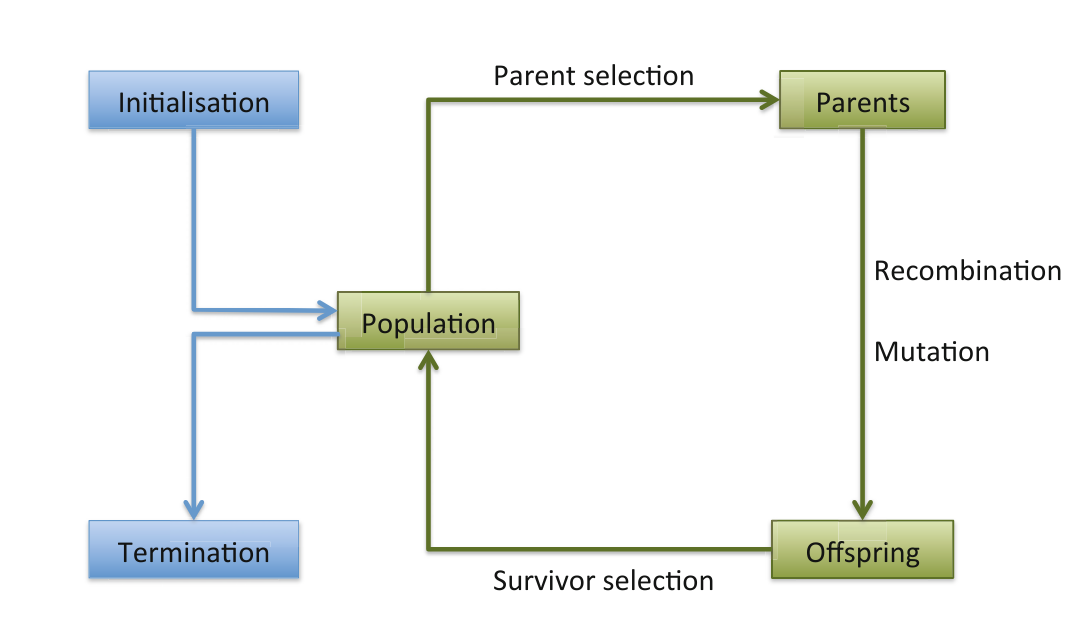
\includegraphics[width=1\textwidth]{EAFlowchart}
\caption{Evolutionary Algorithm Flowchart \cite{Eiben2015}  }
\label{ea}
\end{figure}
This algorithm is the most frequently used for deck building problems \cite{Fludal2017}\cite{GarciaSanchez2016}\cite{GarciaSanchez2018}, although they are optimized in different ways. In GAs, there exists a fitness function that determines the fitness score of an individual that is used to create the next generation, and there is the mutation function which will randomly mutate some individuals (it may or may not improve the fitness of said individual). \\ 
\indent Bjørke and Fludal \cite{Fludal2017} used a genetic algorithm to construct decks for Magic: The Gathering based on a certain pool of cards. Instead of using a fitness function that would calculate the score of a deck, they pitted each deck in that generation against each other in a tournament format using a Magic: The Gathering game simulator, each deck had the same number of games to play and they would select the fittest decks based of their win rate in the tournament. While theoretically, the idea is sound, the time that it took was substantial for an unremarkable win rate (less than 60\%). With 50 matches per deck over 350 generations, it took 43 hours to execute. Due to the time it takes, it would be unusable for players as it would simply take too long.\\
\indent Garcia-Sanchez et al. had a similar approach using lexicographical fitness with a Hearthstone game simulator called \textit{MetaStone}\footnote{\url{https://github.com/demilich1/metastone}}, separating the fitness evaluation into three parts: one part counted the number of victories of in 16 games, another part which determined the deck correctness (no more than 2 duplicates, only 1 legendary, etc...), and the last part was applying standard deviation to the number of victories, it being optimal if the deck won against every opponent \cite{GarciaSanchez2016}. The results were achieved faster much faster and were of a better standard than Bjørke and Fludal's work\cite{Fludal2017}, however, the results were not as high as they could have been, mainly due to the fitness function using \textit{MetaStone's} greedy AI to play. The decisions made by the AI would be greedy and different from that of a human player. The mutation function could also have been touched on, allowing the mutation to make smarter decisions about which cards to mutate. \\
\indent Garcia-Sanchez et al. tackled the problem once again and touched on the mutation function \cite{GarciaSanchez2018}, they developed a \textit{smart mutation} function that would replace a card in a deck with another of a similar cost (roughly ± 1). The results with the smart mutation were overall better than without it. This may solve one of the weaknesses of their previous work\cite{GarciaSanchez2016} but still uses the same greedy simulator heuristic.
\section{Machine Learning}
Machine Learning is a subset of Artificial Intelligence that constructs systems that can learn and improve without the need to be explicitly programmed. Burkov described it as "a subfield of computer science that is concerned with building algorithms which, to be useful, rely on a collection of examples of some phenomenon." \cite{burkov2019} \\
\indent This section of the review will present Machine Learning techniques that have been used or could possibly be used for deck building.
\subsection{Artificial Neural Network}
Artificial Neural Networks (ANN) also known as Neural Networks (NN) for short is an algorithm that was inspired by the biological neural networks seen in brains. They are a group of interconnected nodes or \textit{neurons} typically organised into multiple layers, an input layer, an output and \textit{n} amount of hidden layers. Through many loops known as \textit{epochs}, the NN trains itself using data from datasets to ultimately make a prediction based on given data as an input. Each node is weighted, and these weights are updated throughout the training process increasing the weight of positive output and decreasing on a negative one, allowing the system to make more accurate predictions \cite{3blue1brown}  \\
\begin{figure}[h]
\centering
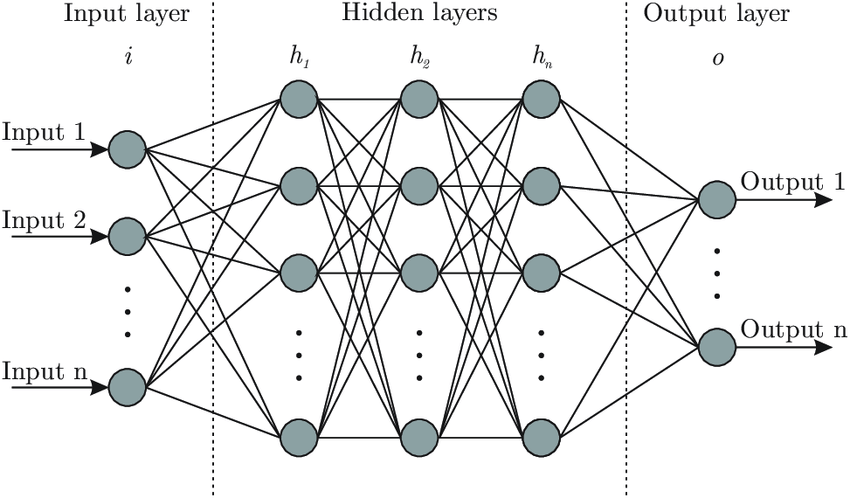
\includegraphics[width=1\textwidth]{ANN}
\caption{Artificial Neural Network architecture \cite{Facundo2017}  }
\label{ea}
\end{figure}
\\
\indent The approach to developing a deck-building AI is done differently than a GA. Ward et al. created a NN that emulated the choices a human would make when drafting a deck from a pool of cards for Magic: The Gathering \cite{Ward2020}. The idea was to select the cards that were chosen by a human in the dataset (target variable). The resulting accuracy on the test set was 65.7\%. The main drawback to this technique is that it requires the data to be clean, since the dataset used was a lot of decks drafted by human players, the data within may be suboptimal or purposefully tampered with, which would cause the AI to build weaker decks. \\
\indent Jakubik attempted a different method by using a NN to predict the win rate of a Hearthstone deck learned by using the results of observed matches \cite{NNWRPrediction}. This was a proposed solution to the AAIA’18 data mining challenge and came second. However, Jakubik's solution was subject to over-fitting, which Hieu Vu et al. tackled during the same challenge, which brought them the winning solution to the AAIA’18 data mining challenge\cite{PredictWR}. They tackled over-fitting by doubling the number of input features (or nodes) to account for the opposing player, they added an extra hidden layer and more test cases to compensate. Jakubik \cite{NNWRPrediction} and Hieu Vu \cite{PredictWR} rely on data of games that have already been played meaning that this method is not suitable for the construction of the decks rather the prediction of the win rate based on games that have been played. Ward et al. paper is the better technique of the three papers to build good decks, however, it requires clean and uncorrupted data.
 
\subsection{Generative Adversarial Networks}
Generative Adversarial Networks (GAN) is an application of generative modeling originally described in 2014 by Goodfellow\cite{NIPS2014}, which is an unsupervised learning task that automatically discovers patterns in the input data that the model can then use to output new examples that could have been drawn from the original data. A GAN uses a generative model to generate a similar output and a discriminator model uses supervised learning techniques to determine the probability of the generative output to be part of the training data\cite{NIPS2014}. The goal of the generative model or \textit{generator} is to create an output that can trick the discriminator into thinking it was part of the dataset. Goodfellow et al. use a fake money analogy: "We can think of the generator as being like a counterfeiter, trying to make fake money, and the discriminator as being like police, trying to allow legitimate money and catch counterfeit money"\cite{NIPS2016}. The GAN trains itself like this until the generator can create something that tricks the discriminator. Figure 1.6 shows the architecture of a GAN\\ 
\begin{figure}[h]
\centering
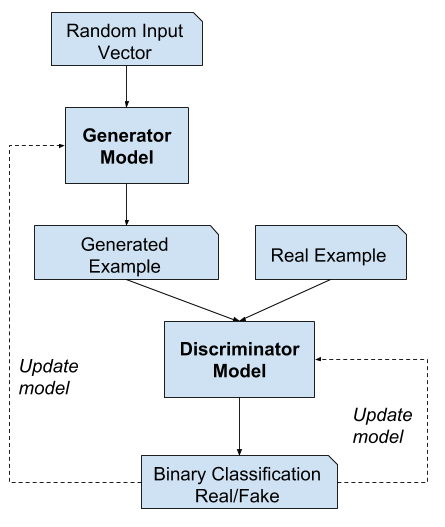
\includegraphics[width=0.5\textwidth]{GAN}
\caption{Generative Adversarial Network architecture\protect\footnotemark}
\end{figure}
\footnotetext{\url{https://machinelearningmastery.com/what-are-generative-adversarial-networks-gans/}}
\\
\indent As of writing this, there have not been any applications of a GAN for building decks. However, Rodriguez Torrado et al. combined a GAN with a procedural content generator to create different playable levels that were randomly generated from the generative model\cite{VGLG}. The GAN struggled to make playable and unique levels when provided a small amount of data. With this paper, it is theoretically possible to apply a GAN in a deck-building context but it will require a large amount of data to provide malleable results. 

\section{Hybrids}
In AI, aspects of a problem to be solved can be optimised through the use of multiple AI. This section of the review discusses papers that have used a combination of machine learning and evolutionary algorithms. The reason why GAs are combined with Machine Learning techniques is that GAs do not require lots of data to function, this allows for uses such as parameter optimization, Sehgal et al.\cite{Sehgal2019} uses GAs to speed up the learning process of their Deep Reinforcement Learning (RL) agent and provided the maximum success rate faster. Such et al. \cite{Such2017} used it for similar work, and stated that is was a competitive alternative to popular RL training techniques. It has also been observed that in the chemical field that the GA could outperform generative models in a discriminator neural network \cite{Nigam2019}, exploring the possibility of an application in GANs. The use of genetic algorithms in hybrid neural networks is mainly for achieving results faster \cite{Sehgal2019}\cite{Such2017}, however in highly parametrized systems the GA tends to struggle to find the optimal combination. \cite{Janikow1993}

%----------------------------------------------------------------------------------------
%	SECTION 3
%----------------------------------------------------------------------------------------
\section{Conclusion \& Final Thoughts}
This literature review has covered existing deck building solutions from Hearthstone and Magic: The Gathering, including evolutionary algorithms, neural networks, and various assistance systems. Potential solutions such as hybrid algorithms and Generative Adversarial Algorithms have also been discussed. Based on this literature review, it has been determined that evolutionary algorithms are the most popular method of tackling the problem therefore the most saturated of new solutions to explore. Machine Learning is a more obscure usage, focusing mainly on win rate prediction and card ranking. Hybrid algorithms and GANs have not yet been used in a deck-building context. In the context of GAs and NNs, they attempt to solve the deck building problem from different perspectives, the GA attempt to build a deck directly and test it in a simulated environment to determine the power of the deck in real-time, whereas the NN focuses on previous data that it uses to predict the power of the deck. They achieve the same goal, however, GAs are more direct and provided concrete results whereas the NN focuses on an indirect prediction from previous use cases. Moving forward this paper will explore solutions within those methods.


\chapter{Requirements}
	%\renewcommand{\labelenumi}{\Roman{enumi}}
	\section{Functional Requirements}
	\begin{enumerate}
		\item{ AI \textbf{MUST} output a legal deck following the rules of Hearthstone. Meaning that a deck should be composed of 30 cards, with no more than 2 duplicates of any card (excluding legendaries, which can only have a single copy).}
		\item AI \textbf{MUST} output a deck following the rules of the "Standard" game mode. Meaning that the AI can only use the classic card set and the latest expansions from the past 2 years.
		\item AI \textbf{MUST} use a generative adversarial network in order to generate a deck. The network will include a generator to create a similar and a discriminator to determine if the deck is part of the dataset.
		\item AI \textbf{MUST} use a dataset of user created decks from the latest expansions in standard format (Rise of Shadows, Saviors of Uldum, Descent of Dragons, Ashes of Outland, Scholomance Academy, Madness at the Darkmoon Faire) collected from Hearthpwn.
		\item AI created decks \textbf{MUST} be tested in a simulator to output a predicted win-rate and determine the playability of the deck versus user created decks. A total of 16 games should be played for optimal results. This will allow for the completion of requirement "f". 
		\item The generated deck \textbf{SHOULD} have a calculated win-rate of over 50\%. Ideally around 60\%, so that the AI can make worthwhile decks. Meaning that the created decks should win at least half of the time, and in an ideal scenario they would win more often than lose.
		\item AI \textbf{SHOULD} output a dataset of decks it generated following the same format as the training data, as to log the output and determine a possible bias.
		\item AI \textbf{SHOULD} be able to generate a deck from a limited collection of cards, so it can be useful to players without access to all cards in Hearthstone.
		\item AI \textbf{COULD} be used in the wild format, making use of all expansions to create competitive decks from a larger pool of cards.
		
		\item An interface \textbf{COULD} be created to accommodate the AI and assist in feature implementation and accessibility of users. 
	\end{enumerate}
	\section{Non-Functional}
	\begin{enumerate}
		\item \textbf{MUST} have written consent from Hearthpwn to scrape data for dataset
		\item Data collected \textbf{MUST} conform to GDPR regulations and be anonymous, since the identities of decks created by users is not needed.
		\item \textbf{MUST} use Python as the programming languages of choice for the access to expansive libraries for data manipulation and AI creation.
		\item \textbf{MUST} use Jupyter notebook as the software for coding the AI. It provides a platform for Python, and the cells are useful for making small changes without having to re-execute the whole program.
		\item Dataset size \textbf{MUST} not be more than 100,000 rows as to decrease time to train and prevent overfitting.
		\item The training process of the AI \textbf{SHOULD} take less than 3 hours, to allow a faster uptime if the AI needs to retrain after an update.
		\item AI \textbf{SHOULD} use card data from the The Hearthstone API on RapidAPI if needed, to collected data such as card effects, images and tribal tags based of the name of the cards.
		\item AI \textbf{SHOULD} use deck data scraped from Hearthpwn to train from using a coded web scraper.
		\item Creation of a deck after training \textbf{SHOULD} not take more than 10 minutes. As to allow the to be quick to use by others whilst allowing for testing time with the simulator and the generation of graphs
		\item \textbf{COULD} generate graphs of performance of decks outputted by the AI and simulators to visualise the training and testing process including the results of the created decks. 
	\end{enumerate}
%----------------------------------------------------------------------------------------
%	BIBLIOGRAPHY
%---------------------
\bibliography{export}


%----------------------------------------------------------------------------------------


\end{document}